\chapter{Resultados y pruebas}
\label{chap:results}
\vspace{0.5cm}

%%%%%%%%%%%%%%%%%%%%%%%%%%%%%%%%%%%%%%%%%%%%%%%%%%%%%%%%%%%%%%%%%%%%%%%%%%%%%%%%
% Objetivo: Exponer los resultados objetivos del sistema                       %
%%%%%%%%%%%%%%%%%%%%%%%%%%%%%%%%%%%%%%%%%%%%%%%%%%%%%%%%%%%%%%%%%%%%%%%%%%%%%%%%

 
\lettrine{E}{n} este capítulo se expondrán los resultados y el funcionamiento de los módulos desarrollados en este trabajo mediante tres aplicaciones de ejemplo.
\section{Ejemplos de uso}
Para probar el correcto funcionamiento de los módulos de interacción, a parte de los ejemplos de desarrollo que se comentaron en el capítulo \ref{sec:InteractionLibraries}, se desarrollaron tres aplicaciones Android que utilizan en conjunto los diferentes módulos de interacción.

\subsection{Simon dice músical}
El primero de los ejemplos desarrollados es un juego educativo musical, similar al juego Simón, en el que los participantes deben repetir una secuencia de colores que se va ampliando en cada iteración de la partida, pero utilizando notas musicales. El objetivo final de este juego es que el usuario consiga asociar los tonos escuchados con la nota músical correspondiente, además de ejercitar la memoria.
En este ejemplo se han utilizado los siguientes módulos:

\begin{itemize}
	\item SoundDispatcherModule: Necesario para el funcionamiento de los módulos de sonido
	\item PitchDetectionModule: Usado indirectamente por el NoteDetectionModule
	\item NoteDetectionModule: Utilizado a la hora de detectar las notas musicales producidas por el usuario.
	\item ClapDetectionModule: Se utiliza para iniciar el juego, una primera palmada prepara al robot y la segunda inicia el juego.
	\item EmotionSoundModule: Diferentes sonidos son reproducidos en función del resultado del juego.
	\item NoteGeneratorModule: Se emplea para generar los diferentes tonos que debe reconocer el jugador.
	\item VoiceProductionModule: Se usa para dar información al usuario y dar una mayor sensación de interacción con el robot
\end{itemize}

Además de los módulos creados en este trabajo, se emplean varios módulos que provee el ROBOBO! Framework:

\begin{itemize}
	\item EmotionModule: Provee la cara del robot, con la posibilidad de cambiar sus expresiones, es la interfaz gráfica que se le muestra al usuario.
	\item DefaultMovementModule: Permite el uso de la plataforma robótica de forma simple, permitiendo el movimiento del robot.
	\item IRobInterfaceModule: Provee un método para obtener la clase IRob, que se emplea para un control más avanzado del Rob, por ejemplo, para utilizar los leds de la base.
\end{itemize}

El jugador inicia la partida dando una palmada, momento en el que el robot pronunciará a través del modulo de voz \enquote{Ready}, una segunda palmada comenzará la partida en si, el robot dirá una frase retando al usuario, por ejemplo \enquote{follow me if you can}, y procederá a reproducir un tono musical. En el momento en el que termine el tono, cambiará la cara dando a entender que está escuchando al usuario, en el momento en el que el jugador termine de producir la nota se comprueba si corresponde al tono original, si coincide el robot realizará una pequeña celebración y volverá a producir tonos, añadiendo uno más a los reproducidos anteriormente. En caso de que el jugador falle, el robot pondrá cara de disgusto, producirá un sonido de abucheo y volverá al estado inicial, esperando a una palmada para iniciar el juego.

En esta implementación del juego, para que tenga una sonoridad agradable, solamente se producen tonos dentro de la escala pentatónica menor de La (figura \ref{fig:pentatonic-scale})

\begin{figure}
	\centering
	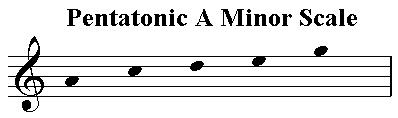
\includegraphics[width=0.6\linewidth]{imagenes/pentatonic-scale-a-minor.jpg}
	\caption{Escala pentatonica menor de La}
	\label{fig:pentatonic-scale}
\end{figure} 

\subsection{Robobo Vigilante}
\subsection{Robobo Mascota}


\section{Problemas conocidos}
\begin{itemize}
	\item La tasa de refresco del módulo \textit{BasicCamera} es baja y varía mucho entre terminales móviles.
	\item El \textit{ColorDetectionModule} puede confundirse si el fondo no es homogéneo, se recomienda usar tarjetas con colores sobre fondo blanco.
	\item El \textit{EmailModule} puede causar el bloqueo de la cuenta de Gmail si esta no es configurada previamente para usar mediante IMAP.
	\item El \textit{TouchModule} requiere el paso explícito de los TouchEvents de la actividad en pantalla.
\end{itemize}
\label{sec:known_issues}
    

